\chapter{Near-bottom turbulence and sediment transport in the Western Baltic 
Sea}
\label{kap-measure}

This study addresses the question whether the deep basins in the Baltic Sea are 
purely depositional or if sediment once settled there can be transported back 
to shallower areas. Field data, including long-term moorings and 
microstructure measurements, from three cruises in three different years 
and seasons has therefore been analyzed to investigate mean current, turbulence 
and suspended sediment concentration. Measurements have been carried out on the 
transition zone from the German shore to the Arkona basin. It is found that 
net onshore transport of suspended matter originating from the Arkona basin 
takes place. Stratification asymmetries in the flow phases of an oscillatory 
up- and down-slope flow have been identified as a possible mechanism for this 
net sediment transport.

\section{Introduction}\label{introdaten}

The investigation of sediment transport patterns and the physical processes 
involved are essential for the understanding and mapping of many near bottom 
biogeochemical processes. Nutrients as well as pollutants are distributed or 
accumulated together with the sediment, which affects benthic communities and 
the exchange of dissolved substances between pore water and the overlying 
water column. Especially in coastal areas, a broad variety of hydrodynamical 
processes affect resuspension, transport, and accumulation of sediments. In 
shallow areas, wind waves govern the sediment dynamics, whilst mean flow, near 
bottom turbulence and interior stratification becomes increasingly important 
during the transition towards the deeper areas further away from the coast.

Due to negligible tidal motions, coastal areas of the Baltic 
Sea provide a good opportunity to study the interplay between waves and 
currents and their effects on sediment transport patterns. A number of previous 
studies have focused on these issues.
In the \textit{Ba}ltic Sea \textit{Sy}stem \textit{S}tudy (BASYS), the 
pathways of fine-grained sediment from the near-shore regions to the deep 
basins were investigated with the help of numerical models and field 
measurements \citep[][]{basys1, basys2, leipe2000}. The research project 
\textit{Dynamic} of \textit{N}atural and \textit{A}nthropogenic 
\textit{S}edimentation (DYNAS) investigated spatially resolved 
resuspension and transport patterns in the whole near-coastal area of the 
south-western Baltic Sea, using a numerical model 
\citep[][]{dynas1, dynas2}. These studies, amongst many others, focused mainly 
on large-scale sediment transport and the identification of erosional and 
depositional areas of the sea floor. 

Naturally occurring small-scale turbulent motions, which are an important 
factor for sediment transport processes, have not been included in the projects 
mentioned above. In \cite{basys1}, critical sediment resuspension thresholds 
have been investigated by creating artifical turbulence directly on 
obtained sediment cores. Direct in-situ measurements of natural near bottom 
turbulence and its relation to sediment parameters have, to my knowledge, not 
been carried out in the Baltic Sea yet. 

Turbulent motions affect the bottom 
shear stress that causes resuspension and determine how 
suspended matter is mixed up in the water column. In the interdisciplinary 
project The \textit{Se}rvice of sediments in German \textit{Co}stal 
\textit{S}eas (SECOS), in which the present study was carried out, these 
small-scale processes were examined with an extensive field program. This 
included ship-based turbulence micro-structure measurements and long-term 
mooring 
deployments. Observations of suspended matter concentration 
from optical backscatter sensors, mean currents, waves, and turbulent 
motions were combined to study the relative effect of these processes on 
sediment transport at a number of key locations. One of the regions where 
measurements were carried out was the 
transition zone from the near-coastal region to deeper parts of the Arkona 
basin north of the island 
R\"{u}gen. This region was considered as a prototypical transition area for the 
investigation of the different processes responsible for the sediment transport 
processes in the Western Baltic Sea. To our knowledge, 
no turbulence measurements with focus on sediment dynamics were carried out in 
this region so far.
 
In addition, this area provides the prerequisites for the occurrence of 
the slope-induced tidal straining process discussed in the previous chapters 
\citep[][]{UmlaufBurchard2011a, 
schulzumlauf2016}. Both the slope of the sea floor and 
interior vertical stratification are sufficient to trigger residual sediment 
transport under an oscillatory current. Although tides are negligible in the 
Baltic Sea, a distinct signal of inertial oscillations with a 
period of approximately 15~h was visible over five day continuous of
current measurements. This setting certainly exceeds the capability of the 
one-dimensional numerical model used in \cite{schulzumlauf2016}, as the slope 
angle is changing and the vertical stratification is greatly enhanced in the 
region of the present halocline, making the problem at least two-dimensional. 
Nevertheless, sediment transport from the basin up the slope could be induced 
by slope-induced tidal straining under the conditions given in this region.
 
 The deep basins in the Baltic Sea, like the Arkona basin, are depositional 
areas. Net sedimentation can be measured, and sediment is transported from the 
coast to the basins \citep[][]{basys1, basys2}. The main question addressed in 
this study is whether this transport is directed purely one way, or if processes 
exist which can transport parts of the sediment from the deep basins back to 
shallower areas.

\section{Study Area}

The general properties of the Baltic Sea have already been discussed in the 
last chapter. Here, a brief introduction to the general hydrodynamic 
processes which govern the current system near the measurement site on the one 
hand, and the sediment distribution on the other is given.

\subsection{Hydrography and dynamics} 

 \begin{figure}[ht]
 \centering
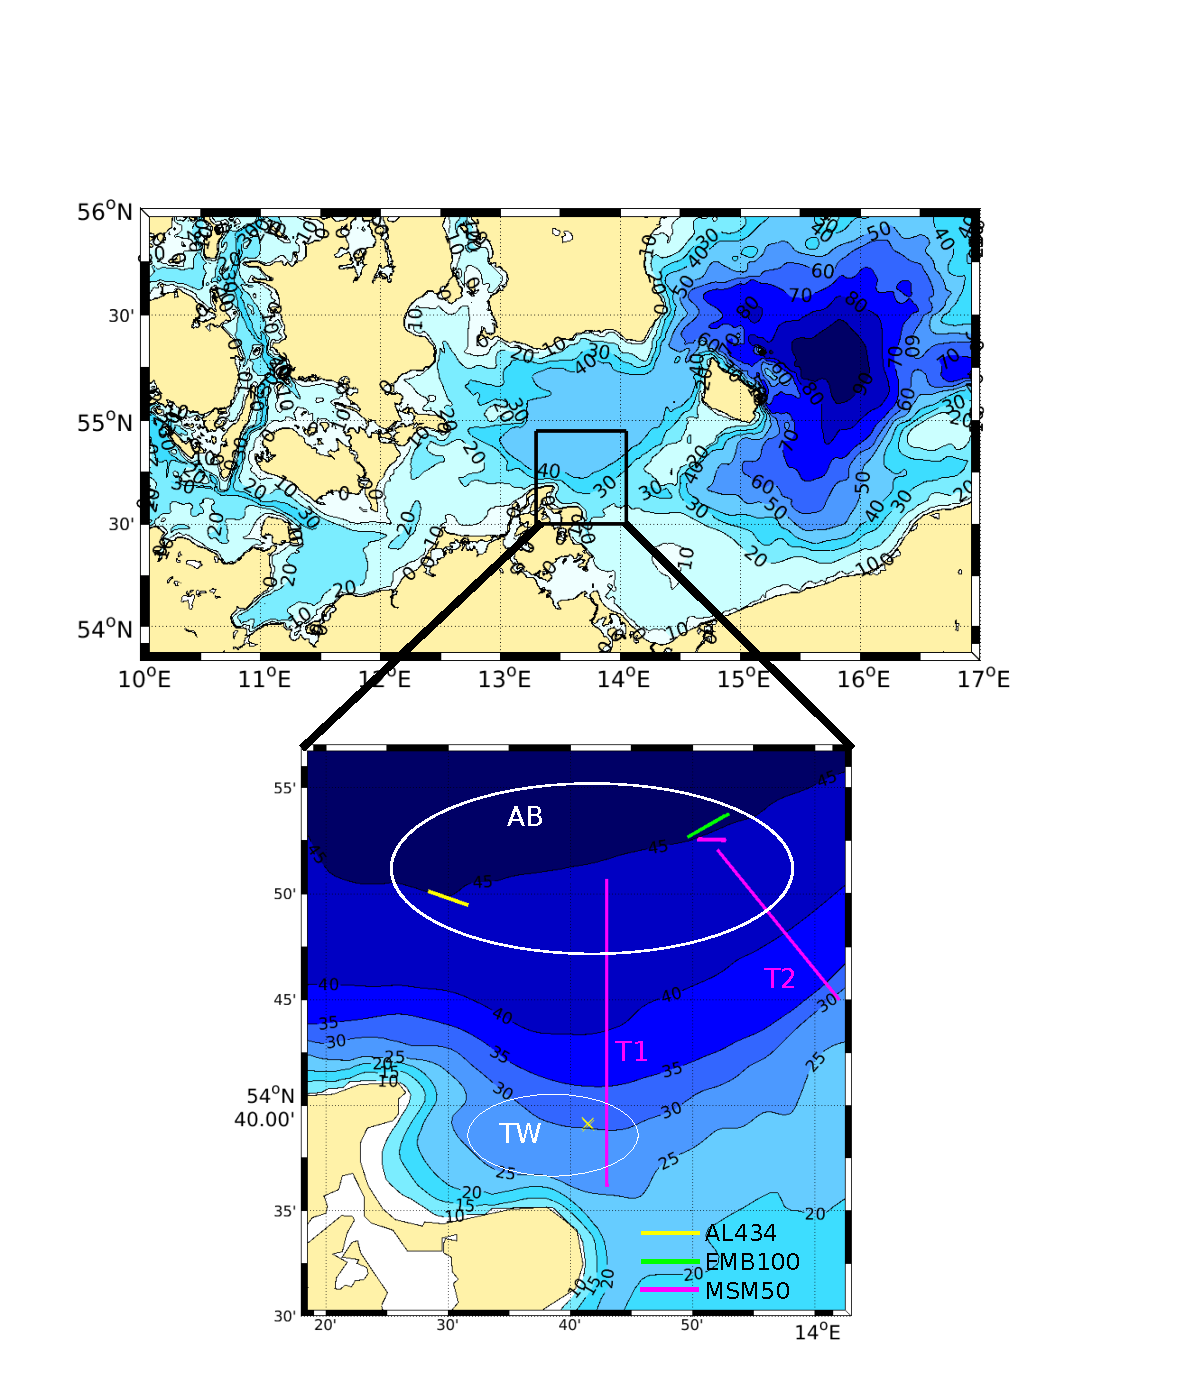
\includegraphics[width=18cm]{bilder/studyarea.pdf}
 \caption{Bathymetric map of the Western Baltic Sea and an enlargement of the 
study area. Deployments during cruise AL434 are indicated in yellow, from 
EMB100 in green and from cruise MSM50 in magenta. Crosses mark the 
position of deployed moorings, lines refer to microstructure profiler 
transects. White ellipses indicate the positions referred to as TW (Tromper 
Wiek) and AB (Arkona Basin), respectively.}
 \label{studyarea}
 \end{figure}
 
In \fig{studyarea}, the bathymetry of the study area and its position in the 
Western Baltic Sea is displayed. The Arkona basin has a maximum depth of 
around 45~m and an extension of nearly 75~km in meridional and 110~km in 
longitudinal direction \citep[][]{lass2005}. \FloatBarrier The flow patterns in 
this area 
have already been investigated with extensive field measurement e.g. in 
\cite{lass1993}. In a study on the Pomeranian Bight (i.e. the shallow area 
connecting the Arkona Basin in the west and the Bornholm Basin in the east and 
where the mouth of the Oder river is located), \cite{lass2001} also investigated 
the study site described here both observationally and with a high-resolution 
circulation model. In addition, the same authors carried out measurements in 
two consecutive winters in the Arkona Basin and analyzed the flow dynamics 
there \citep[][]{lass2003,lass2005}. General information about the deep water 
of the Baltic Sea, and especially the Arkona Basin, are summarized in 
\cite{meier2006}. The dynamics of near-inertial waves in the deep basins 
of the Baltic Sea have been investigated in \cite{vanderlee2011}, with help of 
a field campaign in the Bornholm Basin. These studies give a good insight of 
the flow patterns and dynamics of the area investigated in this study.

From the exchange with the North Sea, dense bottom currents of saline water 
enters the Arkona Basin via the Darss Sill and the Dr{\o}gden Sill (see 
previous chapter). Coriolis effects and bottom friction determine the 
propagation of the saltwater plume, forming a topographically trapped rim 
current which cyclonically encircles the basin and slowly deepens with 
increasing distance from the sills \citep{lass2005}. The saline water is 
diluted and feeds the central pool of dense water in the basin, which 
discharges through the Bornholm Channel (north of the island Bornholm, see last 
chapter). Residence time of the salt water in the Arkona Basin is around 1-3 
months \citep[][]{lass2005, meier2006}.

As inflow events are driven by larger scale wind forcing, this process is not 
steady, and the dense bottom current is modulated by pulses of inflowing 
water and can disappear completely. During an inflow event, baroclinic Kelvin 
waves circumnavigate the basin within 4 days and the halocline is lifted up 
whilst the saline bottom pool is filled with inflowing water. In summer, warm 
inflow events sandwich warm and saline water masses into the halocline. Bottom 
water spills over the Bornholm Channel whenever the height of the bottom pool 
exceeds the depth of the Channel. All this causes the position of the halocline 
to be highly variable in time and also depending on the exact position in the 
basin. For example, after an inflow event in December 1998, the upper laxer of 
the dense bottom water pool was found to be located at 40~m depth in the central 
basin and at about 30~m depth at the southern rim. Three month later, the 
halocline was found to be at around 35~m depth throughout the basin 
\citep[][]{lass2005}.

\begin{figure}[ht]
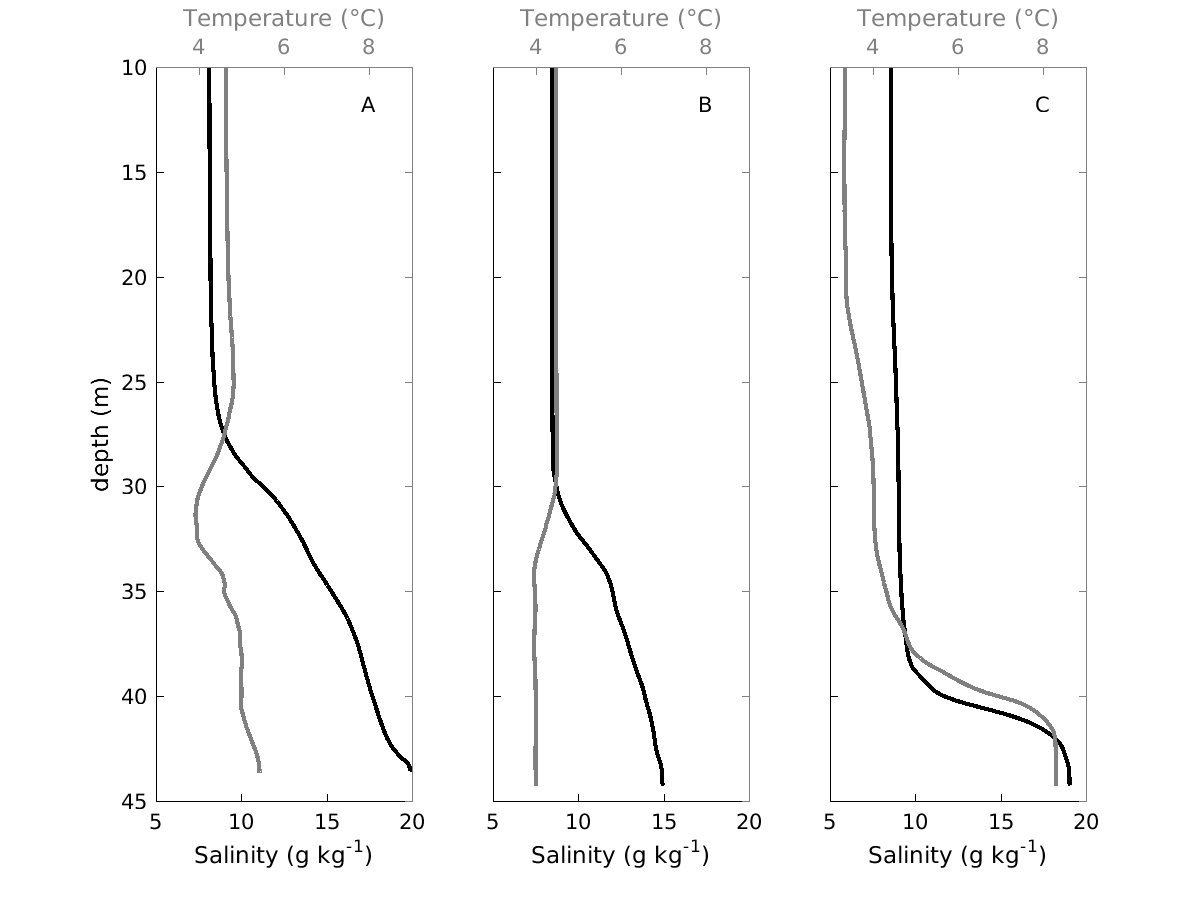
\includegraphics[width=40pc]{bilder/arkona_TS.png}
 \caption{Vertical structure of salinity (black lines) and temperature (gray 
lines) in the Arkona Basin in (a) April 2014, (b) April 2015 and (c) January 
2016. Data are averaged over several microstructure profiles, see caption of 
\fig{abmss} and \tab{mss} in the following chapters for details.}
 \label{TSarkona}
 \end{figure}
 
 This variability is also visible in the data obtained for this study. On 
each of the three cruises microstructure measurements were performed in the 
Arkona Basin (see \fig{studyarea}). In \fig{TSarkona}, vertical profiles of 
temperature and salinity are displayed. The upper layer of the dense bottom pool 
is commonly characterized by a salinity of 11~g~kg$^{-1}$ \citep[][]{lass2005}. 
In April 2014 and 2015 (\fig{TSarkona}a,b), the halocline was located 
relatively high in the water column, at around 27~m and 31~m depth, 
respectively. In January 2015, the interface between dense bottom and overlying 
water is very sharp and positioned deeper in the water column, at around 40~m 
depth. 

Besides the dense bottom current, other flow patterns and hydrodynamic 
processes have been observed in the Arkona Basin, including different 
oscillatory motions that are a prerequisite for slope-induced tidal 
straining (see section \ref{introdaten}). \cite{lass2003} found that the 
barotropic cyclonic motions of the bottom current perform basin wide zonal 
oscillations on timescales of one week. This is in agreement with the findings 
of \cite{lass2001}, that near-shore currents reveal an elliptical motions, with 
the main axis being aligned along the isobaths. North of the island 
R\"{u}gen, the currents are slightly more pronounced towards the east. The 
cross-shore component is generally weaker, but still on the order of 
0.1~m~s$^{-1}$ \citep[][]{lass1993, lass2001}. 

Another factor determining the flow conditions is local wind forcing, 
that causes upwelling and downwelling near the shore. Wind from the east 
drives a long-shore current to the west. In cross-shore direction, Ekman 
transport causes surface flow to be directed seaward. This induces a 
near-bottom return current towards the land \citep[][]{lass1993}. The salt 
water pool in the Arkona Basin is consequently tilted upwards towards the 
southern rim of the basin \citep[][their Fig.\ 11]{lass2003, lass1993}. During 
wind from the west, the situation is reversed. After the wind decays, 
internal seiching motions in the basin are excited driven by the tilted 
density interface of the saline bottom pool.

\cite{vanderlee2011} carried out a study on internal wave mixing in the 
Bornholm Basin and found that inertial oscillations and near-inertial wave 
motions govern the energetics near the slopes of the basin. Density 
stratification and topographic structure are comparable in the Bornholm and 
Arkona Basin, yielding that inertial oscillations also play an important role 
there.

 During cruise AL434, velocity profiles on the southern rim of the Arkona Basin 
were obtained with a moored current meter for more than 5 days (see 
\fig{studyarea}, yellow marks). In \fig{abslope}a, the cross-slope component of 
the near-bottom current (1.7~m above sea floor) is displayed. The time series 
clearly exhibits an oscillatory signal with near-inertial period (around 15~h) 
and an amplitude in the order of 0.1~m~s$^{-1}$. Furthermore, 
in \fig{abslope}b the structure of the water body on a basin-to-coast 
cross-section (indicated with T2 in \fig{studyarea}) is shown. It can be seen 
that the halocline, characterized by very high values of $N^2$, is rather 
aligned with the slope than straight horizontal, and that the extent of the 
dense bottom pool is in agreement with the extent found in the microstructure 
data from the deeper parts of the basin at that time, displayed above in 
\fig{TSarkona}c. The observed stratification strength and the slope angle are 
well within the range for the occurrence of slope-induced tidal straining found 
in \cite{schulzumlauf2016}. 

  \begin{figure}[ht]
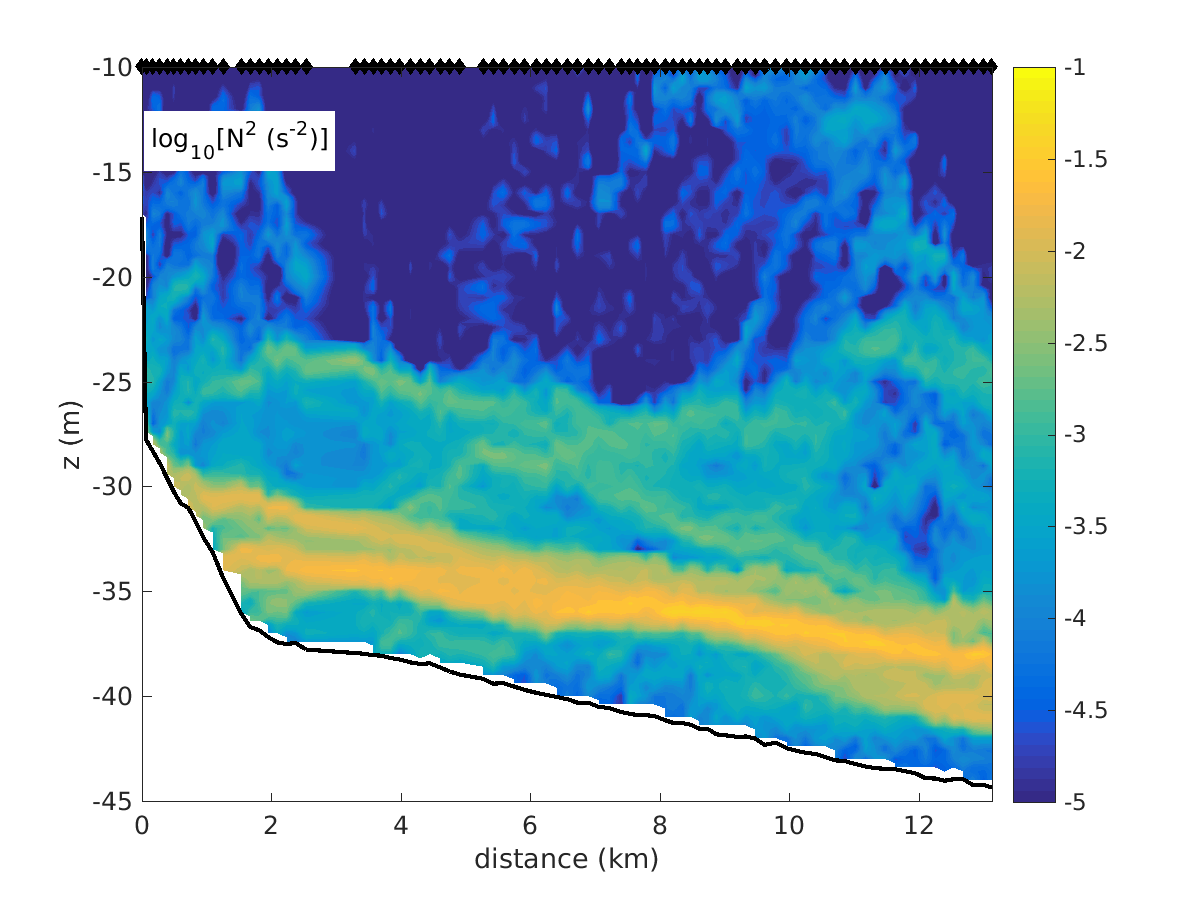
\includegraphics[width=40pc]{bilder/abslope.png}
 \caption{In (a), ca. five days of the cross-slope (i.e. southward) near-bottom 
current are displayed, obtained with a 1200~kHz ADCP in April 2014 (see Tab.\ 
\ref{deployments}, first column). Positive means up-slope. (b) Topographic and 
hydrologic structure in the study area obtained from microstructure transect T2 
(see Tab.\ \ref{mss} and Fig.\ \ref{studyarea}) in 2016. The steep slope on the 
left hand side has an inclination of approximately $5 \times 10^{-3}$, the mild 
slope further to the right of around $7 \times 10^{-4}$. Color indicates the 
buoyancy frequency $N^2$.} \label{abslope}
 \end{figure}

 \FloatBarrier
\subsection{Sedimentology}\label{sedmol}

  Sediment distribution in this area is heterogeneous in the shallow regions 
with predominately medium to fine sand. At water depths below 25 - 30~m in the 
Arkona Basin, sediment is relatively fine-grained and consists homogeneously of 
silt (\fig{tauberkarte}). In the vicinity of TW, a special type of fine grained 
and organically poor sediment is found. 

Previous studies \citep[][]{leipe2000, basys1} found the Arkona Basin to be a 
deposition center for material originating from the shallower areas, with 
accumulation rates of around 2.2 mm/yr. Sediment characteristics in the Arkona 
Basin resemble those of a fluffy layer, implying that sediment is easily 
resuspended with resuspension thresholds of 0.02~N~m$^{-2}$ 
\citep[][, determined with a LABEREX chamber from sediment core 
samples]{basys1}. Current speeds in the order of 
0.05~m~s$^{-1}$ are sufficient to exceed this critical resuspension threshold. 
Due to its low settling velocity of less than $10^{-3}$~m~s$^{-1}$, sediment 
remains suspended for a relatively long period of time. Closer to the coast, a 
fluff layer was found to be present most of the time. Values for critical 
resuspension thresholds and settling velocities were therefore slightly higher 
than the ones observed in the deep parts of the basin. Furthermore, in 
\cite{basys1} wave-induced resuspension was observed six times in three month 
near station TW, and twice near AB.

A consecutive study \citep[][]{basys2} found the 20~m isobath to be the border 
between erosional and depositional sites in this area, suggesting that the 
Tromper Wiek region is depositional as well. These authors also pointed out that 
muddy sediments accumulated below the halocline in this region.

 \begin{figure}[ht]
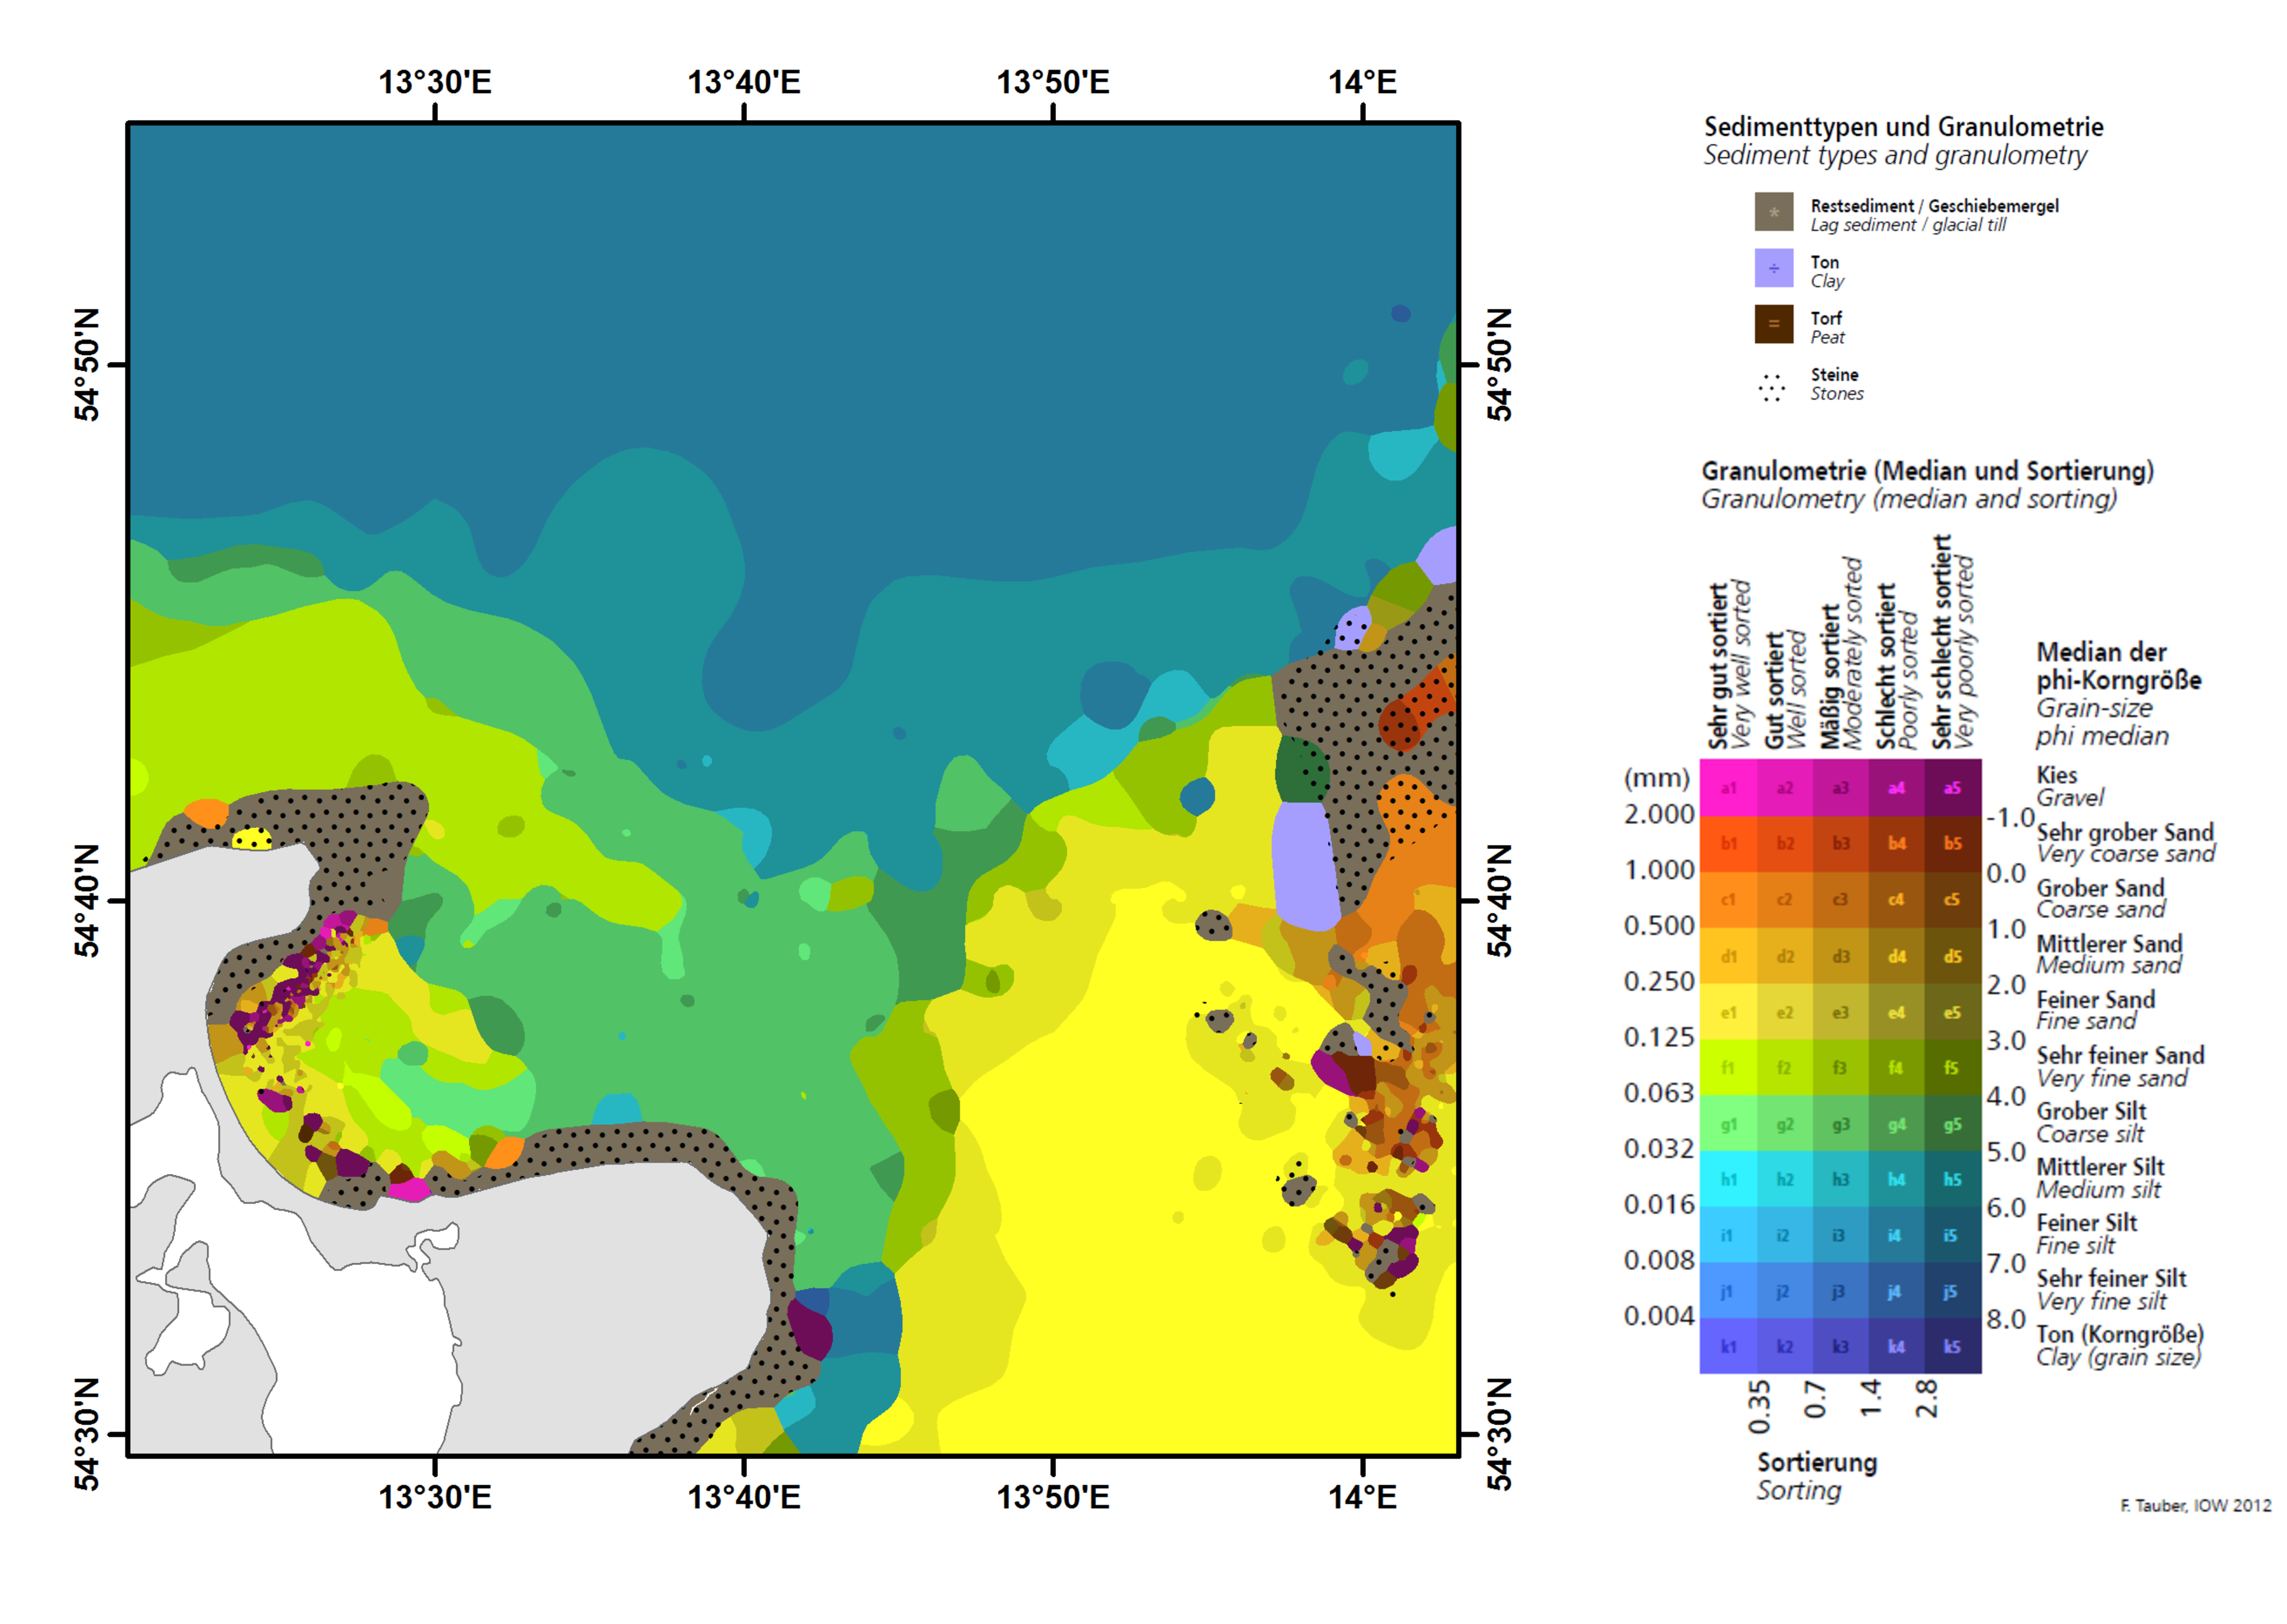
\includegraphics[width=30pc]{bilder/TW.pdf}
 \caption{Sediment distribution in the study area. Data were taken from 
\cite{tauber2012}.}
 \label{tauberkarte}
 \end{figure}

\section{Instrumentation}

Hydrographic and turbulence data were obtained at several locations throughout 
the 
German coastal area during three cruises with R/V \textit{Alkor} in spring 2014 
(AL434, 28.03.-08.04.2014), R/V \textit{Elisabeth Mann Borgese} in spring 2015 
(EMB100, 09.04.-16.04.2015) and R/V \textit{Maria S. Merian} in winter 2016 
(MSM50, 05.01.-29.01.2016). Here, exclusively data obtained in the 
transition zone from the coast off 
the island R\"{u}gen (called Tromper Wiek (TW), around 30~m water depth) to 
the approximately 45~m deep Arkona Basin (AB) are discussed. The exact 
positions of deployed 
moorings and ship-based microstructure profiler transects are indicated in 
\fig{studyarea}, where colors mark the cruise during which the measurements 
were performed.

Three different types of moorings were deployed near position TW during cruise 
AL434. A CTD-Chain consistent of 8 CTD-loggers (MicroCat type SBE37-SM from 
Seabird, USA), tied to a mooring line at intervals of 1 m, starting at 1 m above 
the seabed, with additional optical backscatter sensors (NTU from Wetlabs, USA). 
CTD data were sampled every 10~s, and the backscatter sensor obtained 8 
consecutive samples in 1~s intervals every minute.
Lander 1 was a bottom-mounted instrument frame, equipped with an upward looking 
1200~kHz acoustic Doppler current profiler (ADCP, Teledyne RDI, USA) and a 6 
MHz single-point acoustic Doppler velocimeter (ADV, Vector from Nortek AS, 
Norway).
Lander 2 was a similar bottom frame and, amongst other instruments, equipped 
with an upward looking 600~kHz ADCP (Teledyne RDI, USA).
%and an upward looking pulse-coherent ADCP (Aquadopp HR from Nortek AS, 
%Norway). 

The 1200~kHz ADCP sampled approximately the lowest 15~m of the water column in 
intervals of 0.5~m, with the lowest bin located at 1.6~m above the ground. 
And the instrument was operated in RDI ``mode 12'', 
averaging measured velocity profiles over one set of 4 sub-pings at 300~ms 
intervals every 2~s. 
Velocity profiles over the whole water column were 
obtained with the 600~kHz ADCP, again in 0.5~m intervals with the lowest bin 
located 1.7~m above the ground. Velocity profiles were measured every 2 second, 
averaged from 4 sub-pings in 220~ms intervals. To reduce measurement 
uncertainties, velocity estimates from both ADCPs were averaged over 60~s in 
time. 
The ADV was operated in continuous mode at a sampling rate of 32~Hz. The 
sampling volume was located 1.14~m above the ground.

Deployment times of the moorings, exact deployment position and instrumentation 
are listed in \tab{deployments}.

 \begin{table}
\caption{Deployment duration (UTC), position and instrumentation of the 
moorings deployed during cruise AL434 in April 2014 at position TW (see 
\fig{studyarea}).}\label{deployments}
\begin{center}
% \begin{tabular}{cccc}
% cruise & AL434 (TW) & EMB100 (AB) & MSM50 (TW) \\
%  \hline
%  deployment & 03.04.2014, 07:00 & 14.04.2015, 12:00 & 26.01.2016, 22:00 \\ 
%  recovery & 08.04.2014, 06:00 & 17.04.2015 04:00 & 28.01.2016, 07:00 \\
% \hline
% \hline
% name & CTD-Chain & CTD-Chain & \\
% \hline
% position & 54.6508$^\circ$N 13.6913$^\circ$E & 54.8836$^\circ$N 
% 13.8550$^\circ$E & \\
% \hline
% instruments & 8 CTD-Logger & 10 CTD-Logger & \\
%  & (MicroCat) & (5 MicroCat, 5 RBR) & \\
%  & 1-8~m AG & 1-10~m AG & \\
%  & 2 NTU & & \\
%  & 2.5, 4.5~m AG & & \\
% \hline
% \hline
% name & Lander 1 & Lander 1 & Lander 1\\
% \hline
% position & 54.6528$^\circ$N 13.6908$^\circ$E & 54.8997$^\circ$N 
% 13.8536$^\circ$E & 54.6465$^\circ$N 13.5752$^\circ$E \\
% \hline
% instruments & ADV & ADV & ADV \\
%  & 1200~kHz ADCP &  1200~kHz ADCP & 1200~kHz ADCP \\
%  & MicroCat & MicroCat & SeaCat \\
%  & NTU & NTU & NTU \\
%  & & & miniDOT oxygen sensor \\
% \hline
% \hline
% name & Lander 2 & Lander 2 & Lander 2\\
% \hline
% position & 54.6520$^\circ$N 13.6908$^\circ$E & 54.8836$^\circ$N 
% 13.8563$^\circ$E & 54.6523$^\circ$N 13.5852$^\circ$E \\
% \hline
% instruments & 2~MHz Aquadopp & 1~MHz Aquadopp & 1~MHz Aquadopp \\
%  & 600~kHz ADCP & 600~kHz ADCP & 600~kHz ADCP \\
%  & & SeaCat & SeaCat \\
%  & & NTU & NTU \\
%  & & & miniDOT oxygen sensor \\
%  \end{tabular}
\begin{tabular}{cccc}
& CTD-Chain & Lander 1 & Lander 2 \\
\hline
 deployment & 03.04.2014, 06:54 & 03.04.2014, 06:27 & 03.04.2014, 06:40 \\ 
 recovery & 08.04.2014, 06:19 & 08.04.2014, 06:47 & 08.04.2014, 07:05 \\
\hline
position & 54$^\circ$39.05$^\prime$N 13$^\circ$41.48$^\prime$E & 
54$^\circ$39.17$^\prime$N 13$^\circ$41.45$^\prime$E & 54$^\circ$39.12$^\prime$N 
13$^\circ$41.45$^\prime$E \\
\hline
instruments & 8 MicroCat & ADV & 2~MHz Aquadopp \\
 & 1-8~m AG & 1200~kHz ADCP & 600~kHz ADCP\\
 & 2 NTU & MicroCat & \\
 & 2.5, 4.5~m AG & NTU & \\
 \end{tabular}
\end{center}
\end{table}

Additionally, ship-based microstructure profile measurements were performed 
near position AB with a MSS90-L microstructure profiler (ISW, Germany). The 
instrument contained a set of 
precision CTD sensors (SST, Germany), a fast FP07 thermistor, a turbidity 
sensor, and two airfoil shear-probes (PNS06 from ISW, Germany). The 
sensors were protected with a cage, so profiles were obtained nearly full-depth 
until less than 0.1~m above the ground. During a transect (duration of 1 to 5 
hours) the profiler was continuously operated from the stern of the ship, 
free-falling through the water column with an approximate sinking speed of 
0.5~m~s$^{-1}$, while the ship moved at 1-2~kn. Depending on water depth, one 
profile was measured every 3 to 5 minutes. When multiple transects 
were performed consecutively, the ship turned after the end of each transect 
and was repositioned to the starting position. 
Data processing routines were the same as described in \cite{vanderlee2011}, 
their section 2.2. Data were despiked and averaged to 256~Hz resolution. 
CTD data was binned to 0.1~m intervals in the vertical. Dissipation rates were 
calculated under the assumption of local isotropy in the dissipative subrange 
from the vertical shear spectra and averaged into vertical intervals of 0.5~m.

Position and time of the transects for each cruise are summarized in 
\tab{mss}.

 \begin{table}
\caption{Duration (UTC), start and end coordinate and number of microstructure 
transects performed near AB, total number of profiles in 
brackets.}\label{mss}
\begin{center}
\begin{tabular}{cccc}
cruise & AL434 (2014) & EMB100 (2015) & MSM50 (2016)\\
%  \hline
%  \hline
% position & TW & & TW \\
% start & & & \\
% end & & & \\
% \hline
% duration & 04.04. 16:15 - & & 27.01. 00:00 - \\ 
%  & 04.04. 22:30 & & 28.01. 06:00 \\
% transects & 4 (xx profiles) & &  (9)\\
% \hline
% duration & 06.04. 17:30 - & & \\
% & 07.04. 22:15 & & \\
% transects & 8 (xx profiles) & & \\
\hline
%position & AB & AB & AB \\
start position & 54$^\circ$50.100$^\prime$N 13$^\circ$28.428$^\prime$E & 
54$^\circ$53.689$^\prime$N 13$^\circ$52.694$^\prime$E & 
54$^\circ$52.554$^\prime$N 13$^\circ$52.698$^\prime$E\\
end position & 54$^\circ$49.464$^\prime$N 13$^\circ$31.620$^\prime$E & 
54$^\circ$52.695$^\prime$N 13$^\circ$49.694$^\prime$E & 
54$^\circ$52.548$^\prime$N 13$^\circ$50.508$^\prime$E\\
\hline
duration & 05.04. 16:18 - & 14.04. 16:41 -  & 23.01. 
13:21 -  \\
&  06.04. 01:06 & 15.04. 05:20 & 24.01. 16:41 \\
\hline
transects & 5 (119 profiles) & 5 (184 profiles) & 7 (431 profiles)\\
\end{tabular}
\end{center}
\vskip 0.5cm
\begin{tabular}{ccc}
 on MSM50 & T1 (86 profiles) & T2 (120 profiles) \\
 start position & 54$^\circ$52.079$^\prime$N 13$^\circ$52.036$^\prime$E & 
54$^\circ$36.143$^\prime$N 13$^\circ$43.012$^\prime$E\\
 end position & 54$^\circ$44.992$^\prime$N 14$^\circ$02.022$^\prime$E & 
54$^\circ$50.711$^\prime$N 13$^\circ$43.009$^\prime$E\\
 duration & 24.01. 19:28 - 24.01. 23:42 & 28.01. 09:45 - 28.01. 17:05 \\
\end{tabular}


\end{table}

\section{Observations}

Obtained data are shown in the following, starting with measurements from the 
deep parts of the Arkona basin to understand the structure of the water 
column there. After that, a 13~km turbulence microstrucure profiler transect 
onshore towards shallower areas is discussed. Finally, data from moored 
instruments deployed near TW for several days are displayed and analyzed.

\subsection{Arkona Basin}

 During each of the three cruises AL434, EMB100 and MSM50, microstructure 
profiler measurements were performed in the Arkona Basin. \fig{abmss} shows the 
profiles of 
dissipation rate and turbidity, averaged over all profiles obtained in the 
basin, for each cruise. A turbulent bottom boundary layer (BBL) is visible in 
all three profiles, ranging from 1 to 5 m thickness. 
Turbidity is enhanced in the BBL, but not above, suggesting that the suspended 
sediment causing this turbidity originates from the sea floor. As these 
measurements were performed over three years and in different 
seasons, it is most likely that this turbid, very sharply defined BBL is 
constantly present in the Arkona Basin.

   \begin{figure}[ht]
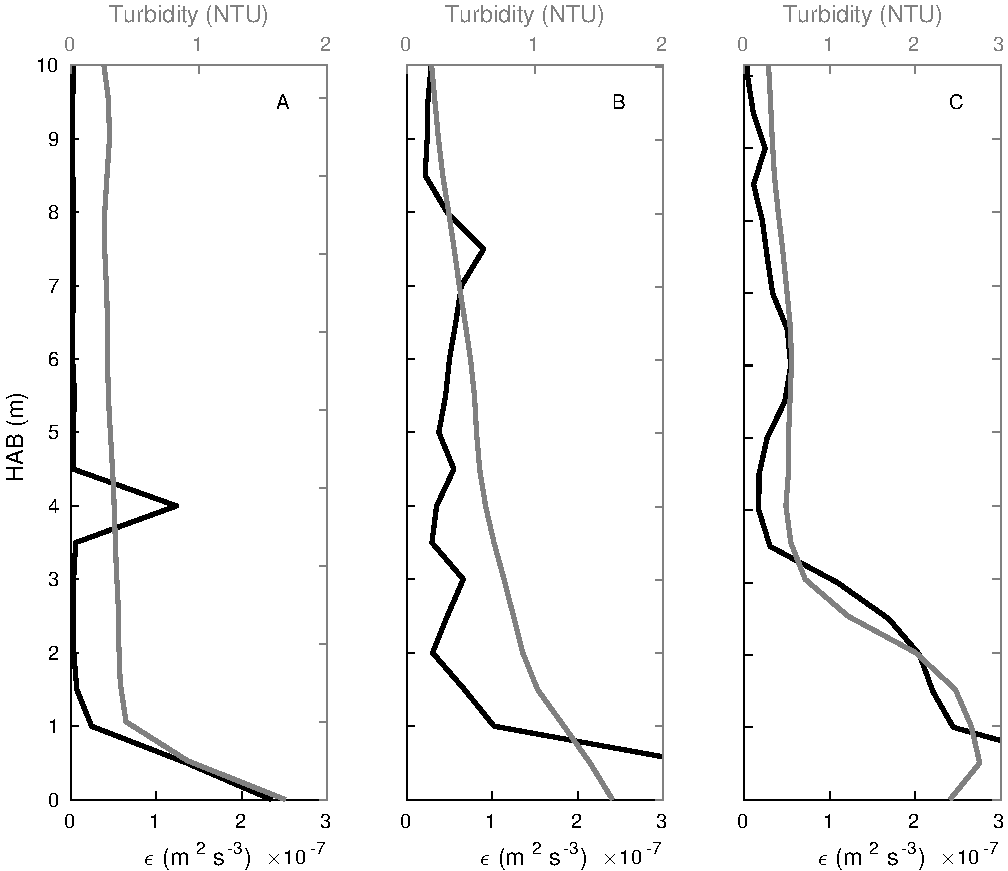
\includegraphics[width=15cm]{bilder/arkona_mss.pdf}
 \caption{Turbidity (gray lines) and dissipation rate (black lines) from all 
microstructure transect performed in the Arkona Basin. Displayed data are the 
average over (a) a total of 119 microstructure profiles obtained during 5 
transects on 05 April 2014 on cruise AL434 were averaged, (b) 184 profiles from 
5 transects on 14-15 April 2015 on cruise EMB100 and (c) 431 profiles from 7 
transects on 23-24 January 2016 on cruise MSM50. Only the lowermost part of 
the water column is displayed here.}
 \label{abmss}
 \end{figure}

The above yields that, on the one hand, suspended sediment transported to the 
Arkona Basin does not necessarily settle there, but is either held in 
suspension or occasionally resuspended and mixed into the turbulent BBL. This 
is in agreement with previous studies that found the sediment in the basin to 
be fluff-like, easily resuspended and slowly settling, see section 
\ref{sedmol}. On the other hand, this reservoir of fine grained 
suspended sediment has the potential to be advectively 
transported across the rim of the Arkona Basin into the shallower areas by 
onshore currents. Under the conditions of present oscillatory currents, 
interior vertical stratification and a bottom slope discussed in the previous 
sections, the Arkona Basin could be a source of sediment to be transported 
up-slope in the process of slope-induced tidal straining.

\subsection{Transect from basin to the coast}

In \fig{transect} it is visible how the water body is structured along the 
slope from the basin onto the coast. A sharp halocline separates a turbulent 
BBL of approximately 5~m thickness from the interior. This 
data was obtained in January 2016. At the southern end of the transect, where 
the slope angle steepens, the halocline is widened where it approaches the sea 
floor. 

The boundary layer is generally turbid. Turbidity is more patchy towards the 
shallow areas, but high values are confined to the bottom boundary layer, 
so no suspended matter is mixed across the halocline. This indicates again that 
turbidity is caused by material originating from the sea floor and held in 
suspension by turbulent motions in the BBL.

The turbulent dissipation rate is also enhanced in the BBL. In the area where 
the halocline encounters the sea bed on the steep slope, dissipation is 
suppressed by the high stratification. Further up the slope, right above the 
halocline, there is again an area with greatly enhanced dissipation. This 
yields that sediment could be resuspended locally when the halocline is 
advected up the slope. This is supported by slightly enhanced turbidity values 
in this region. However, measured turbidity below the halocline exceeds these 
values by more than a factor of two.

Isolines of salinity (please note that salinity mainly determines the density 
in this region) below the halocline are tilted towards the bottom, consistent 
with the observations of boundary layers over sloping topography in e.g. 
\cite{Lorkeetal2005a}. Shear induced convection and, in the presence of an 
oscillatory current, residual (upslope) sediment transport as described in 
\cite{schulzumlauf2016} is consequently within the realms of possibility here.

\begin{figure}[ht]
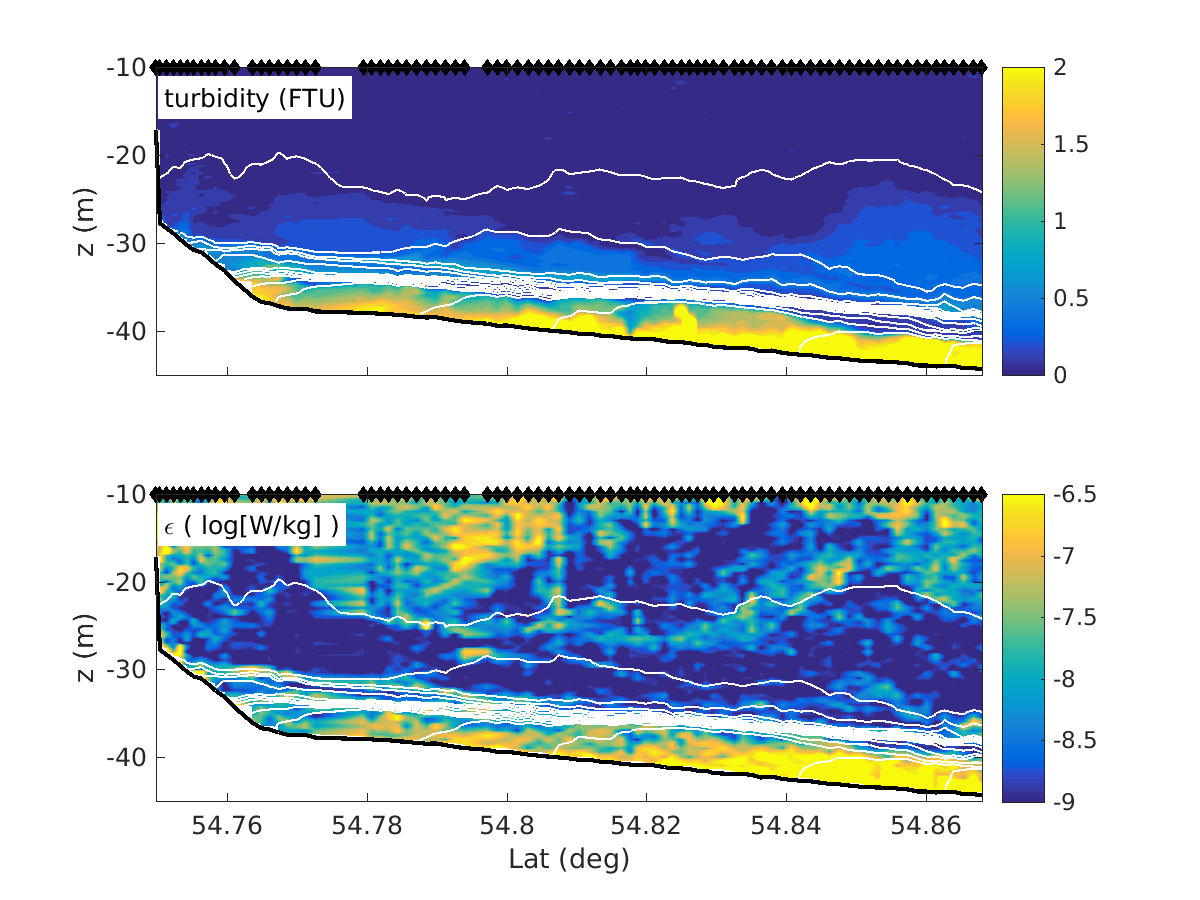
\includegraphics[width=40pc]{bilder/abtrans.png}
 \caption{Turbidity and dissipation rate from the microstructure transect T2 
in January 2016. White lines indicate levels of equal salinity.}
 \label{transect}
 \end{figure}
 
 Although this transect is just a snapshot of the situation in January 
2016, there are several indicators that these conditions are usually present 
here: Turbulent and turbid boundary layers have been visible on all 
microstructure transects in the Arkona basin in three years (see above section), 
and the regional halocline is constantly present, although the extension 
of the dense bottom water pool might differ. Consequently, this transect gives 
an idea of the structure of the water column along the basin to coast transect.
  
\FloatBarrier
\subsection{Tromper Wiek}

In the data from the onshore transect in the last section, it was visible that 
high turbidity values, present throughout the BBL, reach out to water depths 
well below 35~m. In this section, data from instruments deployed at 29~m, 
resembling the shallow end of the transect, were displayed. This data was 
obtained in April 2014, nearly two years before measurements for transect T2 
were performed. However, as the structure of the water body was similar during 
all three cruises, the general situation during the two measurement is 
presumably comparable.

 \begin{figure}[ht]
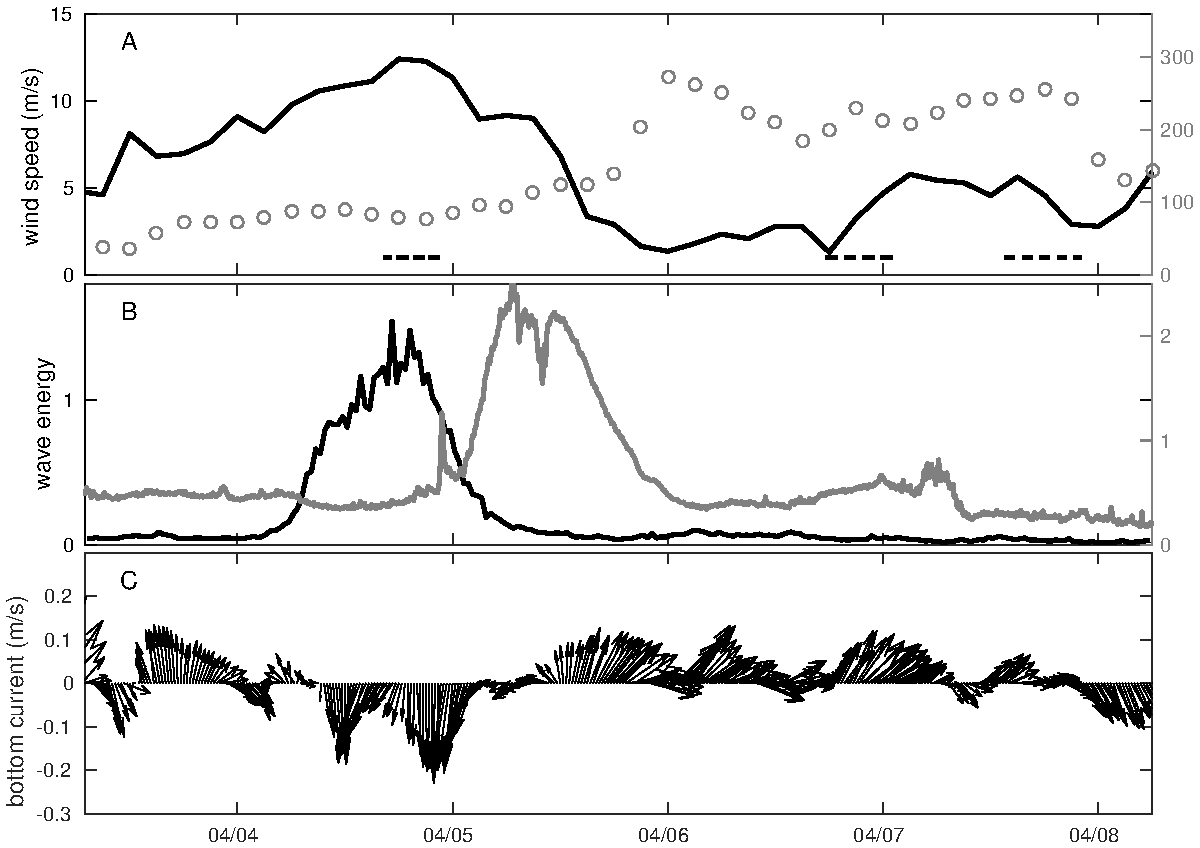
\includegraphics[width=15cm]{bilder/al434tw.pdf}
 \caption{(A) Wind speed and direction from the hindcast of the German Weather 
Service, (B) wave energy and turbidity and (C) direction of 
near bottom current, all obtained with Lander 1 during the deployment at TW on 
cruise AL434 (April 2014). Each black horizontal line in (a) indicates a 
microstructure transect carried out in the vicinity of the deployed mooring.}
 \label{tromperwiek}
 \end{figure}
 
During the 5 day instrument deployment a wind event with wind 
speeds up to force 7 and up to 4 m wave height was captured, followed by a calm 
period (\fig{tromperwiek}a). In \fig{tromperwiek}b the variance of the 
horizontal velocity components, which is proportional to the kinetic energy 
contained in the waves, is displayed. Therefore, data from the ADV (obtained 
at circa 1.2~m above the sea floor) was despiked \citep[][]{goring2002} and 
filtered for wave periods between 2 and 20 seconds with a second order 
Butterworth bandpass filter. Although wave energy was maximum in the afternoon 
of 04 April 2016, the peak in turbidity was not reached until late morning of 
05 April. This suggests that local resuspension during the wind event did not 
occur, but that a turbid water mass was advected to the measurement site. 
Near-bottom currents (\fig{tromperwiek}c) were directed south during the 
relevant period, i.e. water from deeper parts was advected up the slope.
\FloatBarrier
 
 This advection of saline water near the bottom was likely triggered by the 
local wind 
forcing. Strong easterly wind causes Ekman transport to the north (i.e. 
offshore) in the surface layer \citep[][]{lass2001}, \textbf{You could compute 
the Ekman transport from the wind stress, and devide the result by the observed 
surface layer thickness. This would yield an Ekman-related velocity that you 
could compare to your observations.} which is visible in the 
velocity data from the 600~kHz ADCP mounted on Lander~2, displayed in 
\fig{adcp600}\footnote{Corrupted velocity measurements in the uppermost part of 
the water column during 04 April coincide with the periods when strong surface 
waves were recorded with the ADV. These problems most likely originate from 
air bubbles entrained by breaking waves.}. The near-bottom return current below 
17~m depth exhibits a clear near-inertial signal, super-imposed on a southerly 
(i.e. onshore) mean current during the storm. Maximum onshore bottom currents 
were reached by the beginning of 05 April. After wind collapsed and changed 
direction at the end of 05 April, the surface currents 
first decayed and then reversed to southerly directions. Near-bottom 
currents remained unsteady with a mean easterly component. This is more clearly 
visible from \fig{tromperwiek}c.

 \begin{figure}[ht]
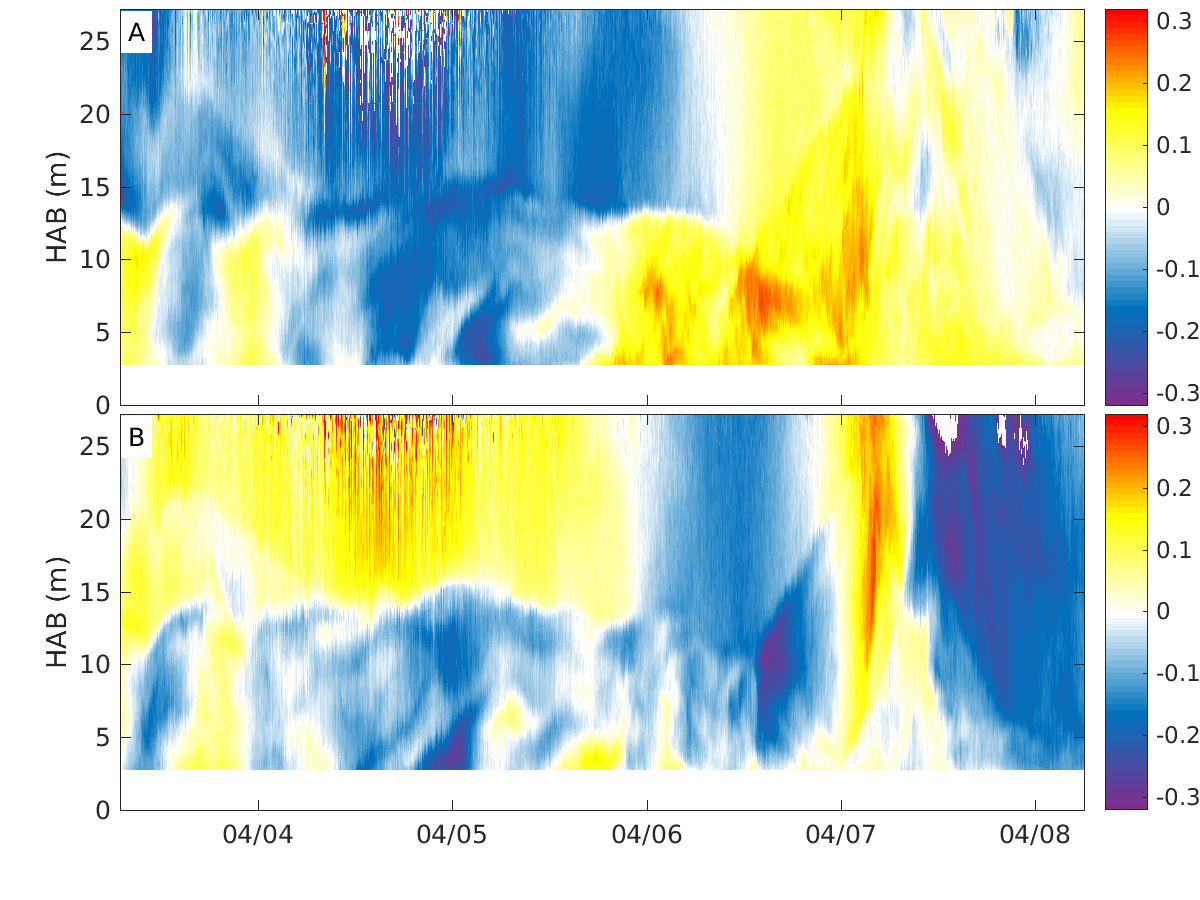
\includegraphics[width=40pc]{bilder/adcp600.png}
 \caption{Contour plots of the (a) east and (b) north component of the 
current velocity, obtained with the 600~kHz ADCP on 
Lander 2 during the deployment at TW on cruise AL434 (April 2014).}
 \label{adcp600}
 \end{figure}

 In the CTD Chain data in \fig{ctdchain} an increase of the 
near-bottom salinity is visible, accompanied by increasing turbidity, starting 
in the 
afternoon of 04 April. The increase in turbidity is clearly linked to the 
increase of salinity, supporting the idea that turbid water is advected to 
position TW from deeper 
regions. Furthermore, salinity data in the record reaches a level that 
resembles the saline bottom waters in the Arkona basin below the 
halocline (see \fig{TSarkona}). This indicates that upwelling 
tilted the halocline, lifted it up in the south and saline bottom water 
reached far upslope onto the shore.

 \begin{figure}[ht]
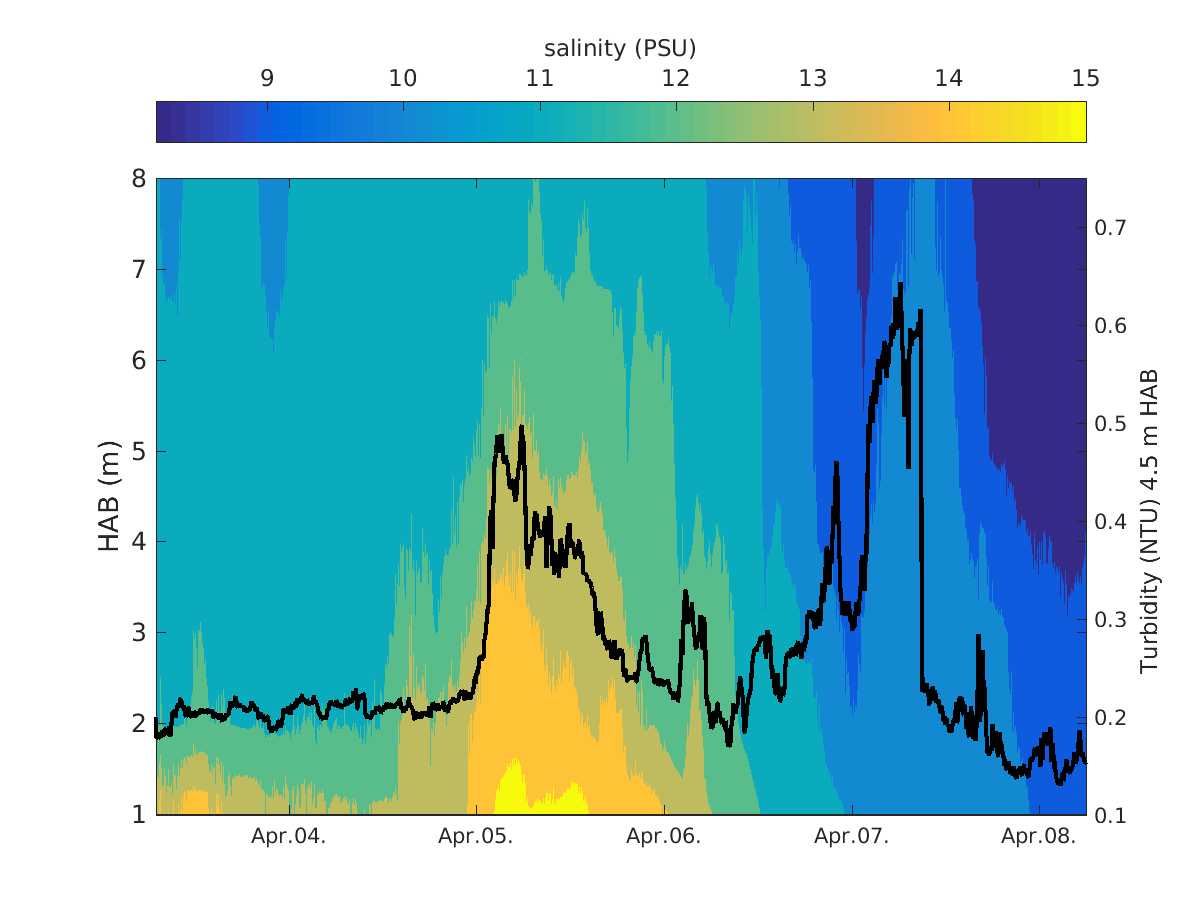
\includegraphics[width=15cm]{bilder/ctdchaintw.png}
 \caption{Salinity data obtained from the CTD Chain deployed at TW 
during cruise AL434 (see \tab{deployments}).}
 \label{ctdchain}
 \end{figure}

\FloatBarrier
\section{Discussion}

This study focusses on finding processes which can transport sediment upslope 
from the deep basins back to shallower areas. It was found from the 
microstructure measurements in the Arkona basin, that in spite of the depth and 
therefore the absence of wave-induced resuspension, a layer of 
suspended fine-grained sediment is present near the bottom. This yields that 
sediment that is transported into the basin can be held in suspension there 
or can be resuspended once it is deposited there.

It was furthermore found that this turbid and turbulent BBL is present 
everywhere 
along the slope, confined by a regional halocline. This near bottom pool of 
saline water with high concentrations of suspended matter is not in rest, but 
advected up- and down the slope by upwelling events and inertial oscillations. 
Sediment originating from the deep parts of the basin can therefore be 
transported on-shore over several kilometers. In the upwelling situation 
discussed above, the integrated near bottom velocity yielded an up slope 
transport over a distance of more than 8 kilometers in less than 24 hours. 

What can not be answered from the observations is whether suspended sediment 
that is transported up the slope settles there and a net upslope transport of 
sediment occurs. A process that induces net sediment transport across sloping 
topography is slope-induced tidal straining. The prerequisites for this 
process, namely vertical stratification, sloping topography and an oscillatory 
current, are all present in the study area. 

From the non-dimensional description of the process in \cite{schulzumlauf2016}, 
it can be inferred which settling velocity, and consequently which kind of 
sediment, 
is favored for up-slope transport. Sediment transport was found 
to be enhanced for non-dimensional settling velocities of $P= w_s \slash U = 
10^{-2}$. Here, $w_s$ is the settling velocity of suspended sediment and $U$ 
the magnitude of the oscillatory flow. Cross-slope flow velocities are in the 
order of 0.1~m~s$^{-1}$ in this region \citep[][]{lass1993}, yielding that 
sediment with a settling velocity of $w_s=10^{-3}$~m~s$^{-1}$ is favored for 
up-slope transport under the conditions investigated in this study. After 
Stokes law, this settling velocity corresponds to medium to coarse silt. As 
visible in \fig{tauberkarte}, this is exactly the sediment present in this 
area. Along the transect T2, indicated in \fig{studyarea}, sediment 
distribution ranges from fine silt in the basin to coarse silt near the shore. 
Additionally, sorting of the sediment is better near-shore than in the basin. 
Both indicates the occurrence of residual sediment transport by slope-induced 
tidal straining here.

Another indicator for sediment transport out of the basin is the distribution 
of mercury in this region. In the Arkona basin, ammunition was dumped during 
World War II. This resulted in a heavy contamination of the sediment with 
mercury. As visible in \fig{hg}, the dumping site in the eastern part of the 
Arkona Basin can be identified from mercury concentrations of over 400~$\mu$g 
kg$^{-1}$. The near bottom mean flow by saline North Sea water progressing 
through the basins is from west to east here, which explains the spreading of 
mercury to the east. The cyclonic rim current can distribute mercury 
contaminated sediment along the rim of the basin. But mercury concentrations 
are also enhanced in shallower parts of the basin, yielding that sediment is 
also transported from deeper to shallower parts, across the isobaths. One 
possible mechanism inducing this transport is slope-induced tidal straining.
   \begin{figure}[ht]
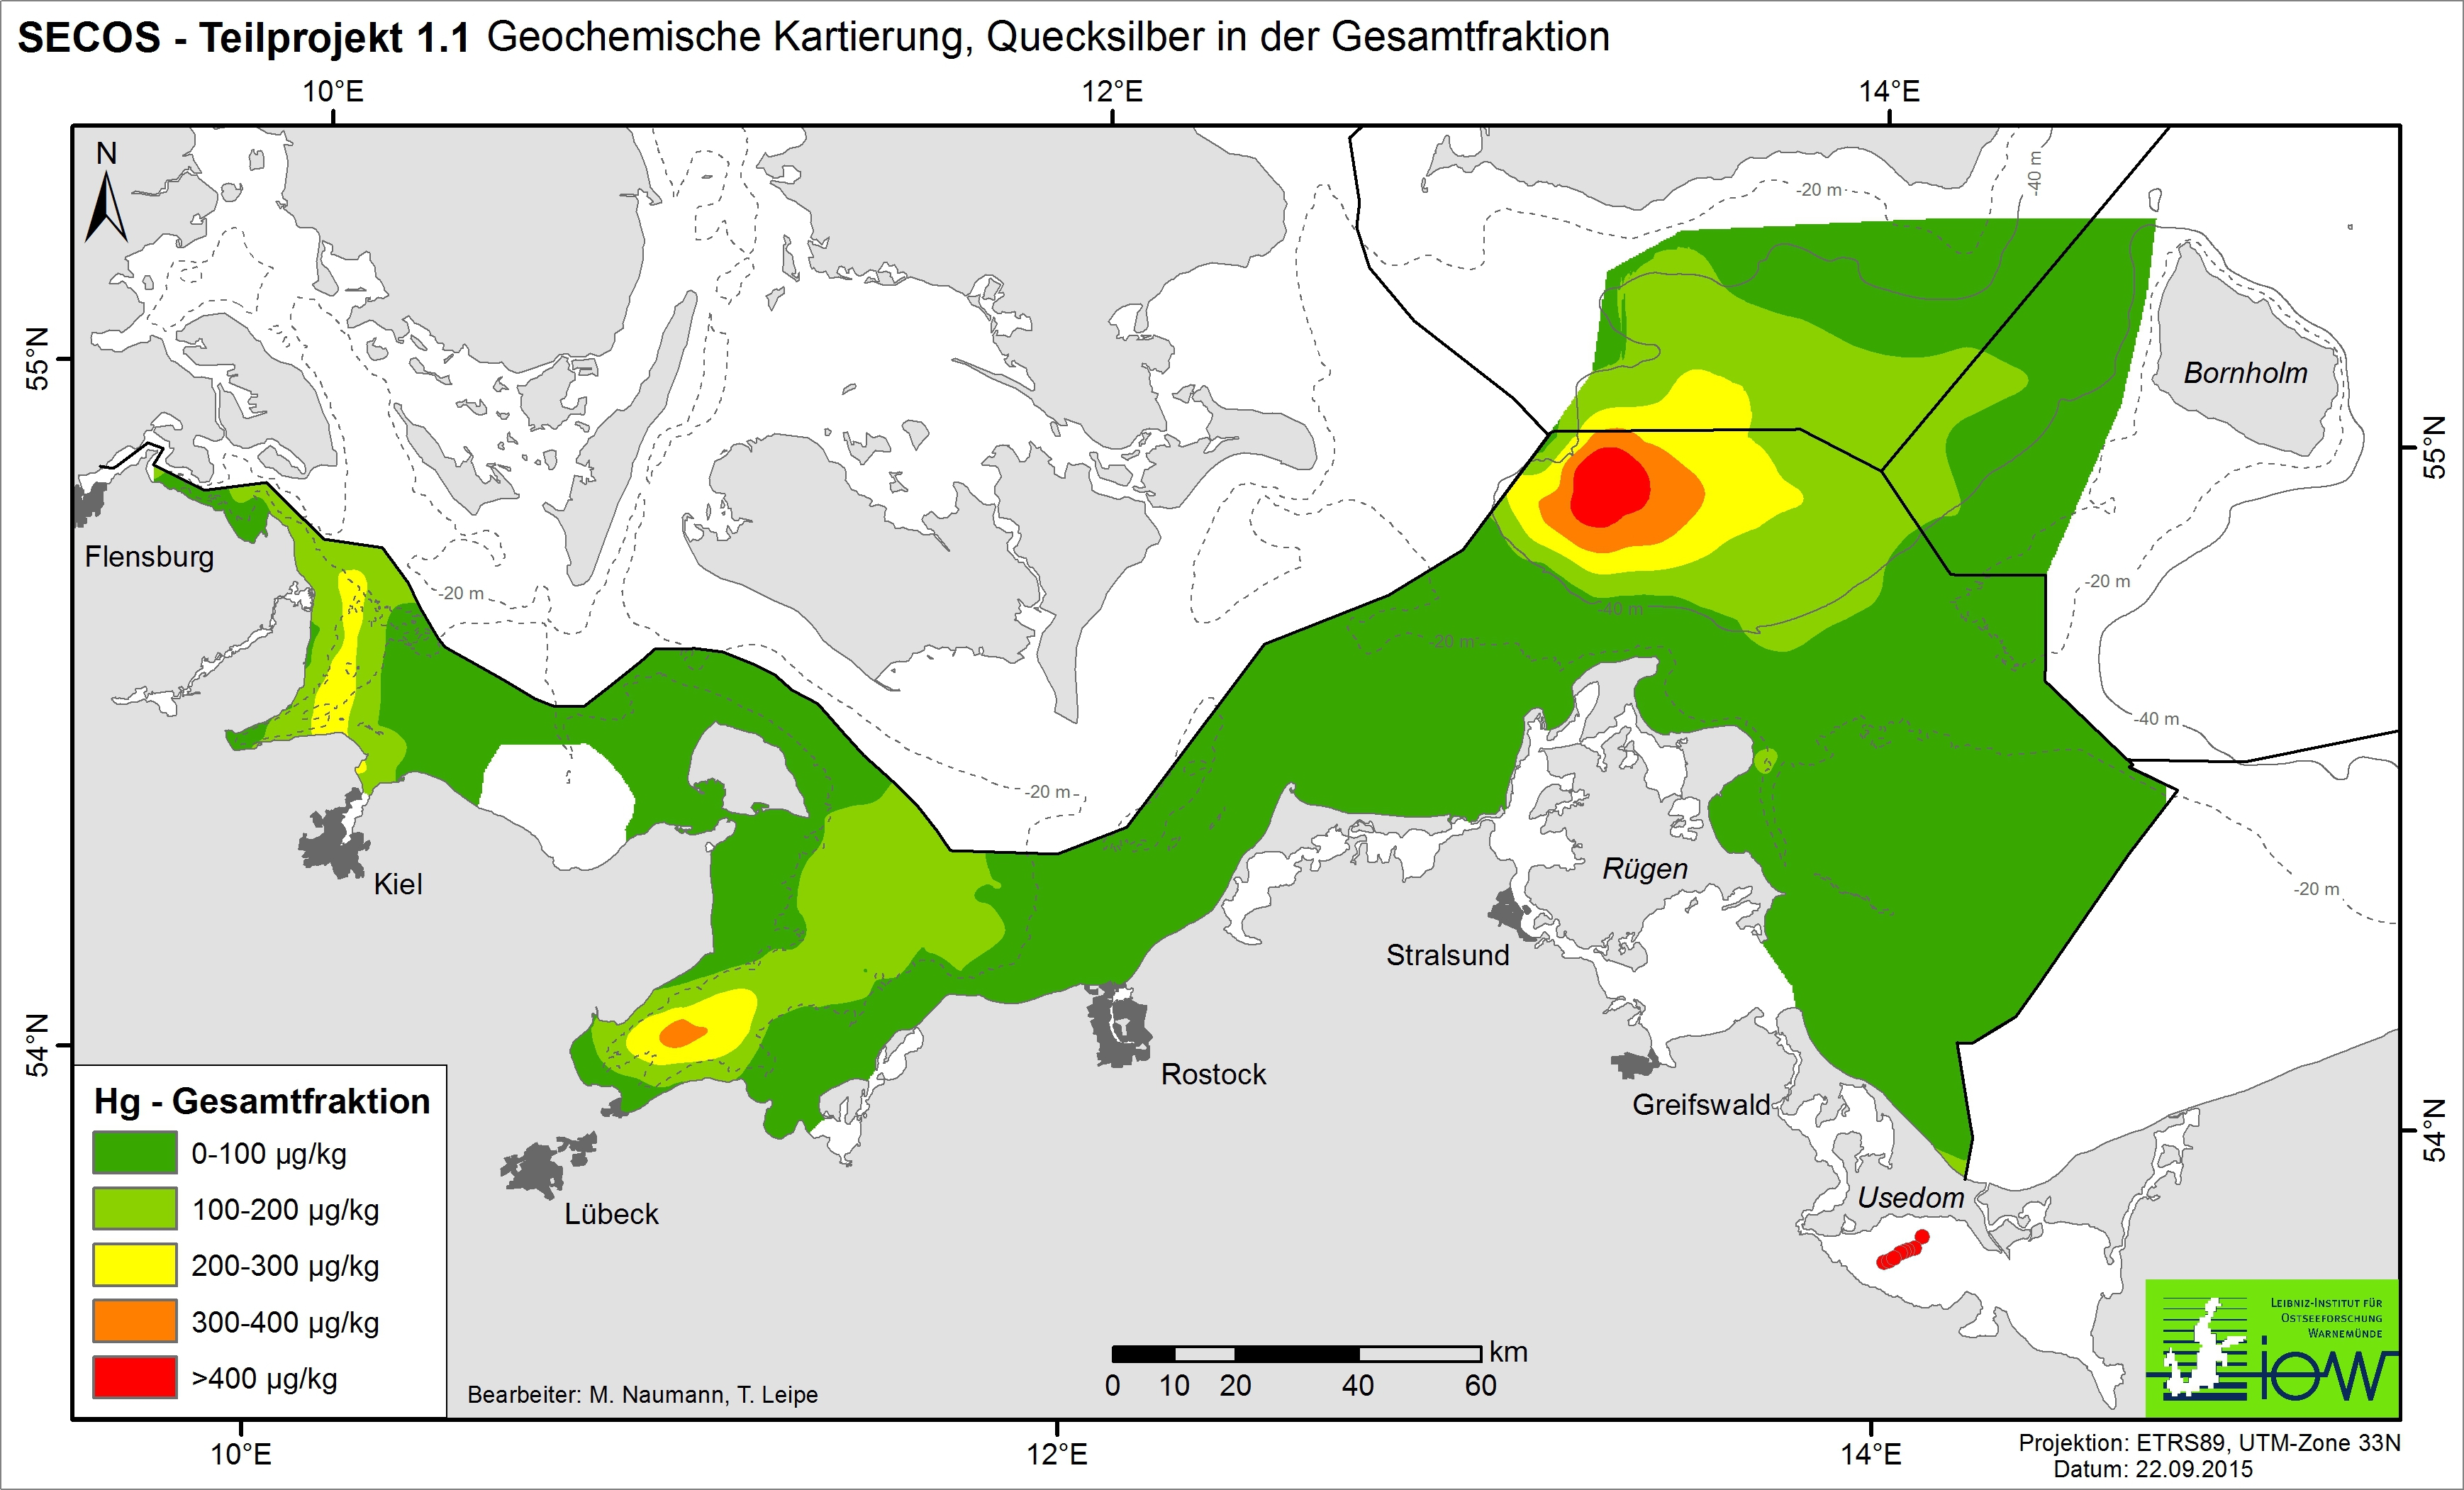
\includegraphics[width=15cm]{bilder/HG_GF.jpg}
 \caption{Mercury concentration in the sediment. Courtesy of Michael Naumann, 
reprinted with permission. [ABKLÄREN UND BESSERE KARTE?]}
 \label{hg}
 \end{figure}
 
\section{Conclusions}

One of the most important findings of this study is that sediment once 
deposited in the Arkona basin can be transported back onshore. 
This yields that fine-grained sediment from all the deep basins in the Baltic 
Sea, which are considered to be purely depositional, can be exported to 
shallower areas. This has great implications on the distribution of pollutants, 
like the mercury originating from the ammunition dumping site in the Arkona 
basin. Pollutants accumulated in the deep basins are not confined to remain 
there, but can spread towards shallower areas where they can endanger the local 
biosystem.

Several different mechanism cause sediment transport in the Arkona basin. 
Firstly, the mean flow of 
the dense bottom current spreads suspended sediment to the east while it 
propagates through the basin structure of the Baltic Sea. Additionally, the 
cyclonic rim current distributes sediment along the isobaths inside the basin. 
Secondly, upwelling tilts the bottom water pool towards the shore and saline 
water from the deep is advected up the basin slope, accompanied by 
suspended sediment originating from the deep parts of the basin. From the data, 
it can not be determine whether this advected sediment is deposited in the 
shallower parts, or if it disappears to the deeper areas again along with the 
saline water mass. Finally, evidences are given that oscillatory currents 
in cross-slope direction, which have been identified not only in our 
observations, can cause a residual sediment transport induces by asymmetries in 
stratification and consequently vertical turbulent mixing as described in 
\cite{schulzumlauf2016}. Observed slope angle and vertical density 
stratification are well within the range which promote up-slope sediment 
transport. Sediment distribution on the transect from basin to the coast is in 
agreement with the type of sediment (characterized by sediment settling 
velocity) that would be favored for up-slope transport under the observed 
conditions. Furthermore, the results found in section \ref{kap-jgr} yield that 
a dominant along-slope velocity component, which is present here, does not 
hinder the residual up-slope sediment transport.

Even though the occurrence of residual sediment transport by slope-induced tidal 
straining can not be definitely proven from the observations, many indicators 
for this process are given. Conclusively, the transport 
mechanism described in \cite{schulzumlauf2016} is likely to take place under 
the given circumstances in the Arkona basin and can explain not only the 
spreading of mercury but also the distribution of sediment in this area.